






\subsection{Nearest particles arrangements}
\begin{itemize}
    \item Problematic : "How the particles are arranged relative to each other"
    \item Show : "How to compute the Radial and azimuthal probability density function : $P_{nst}(r)$  and $P_{nst}(\theta)$"
    \item  Conclusion on $P_{nst}(\theta)$ : "We observe that the particles pair becomes oriented with increasing $Ga$ and decreasing volume fraction.
    \item  Conclusion on $P_{nst}(r)$ : "We observe that the particles pair becomes randomly arranged for high $Ga$ but in average they are rather spaced from each other" 
\end{itemize}
\tb{Je me demande si cette section est vraiment utile .... car elle n'apport pas d'explication supplementaire a la drag force ni aux fluctuations, c'est peux être mieux de garder ca pour l'article qui traîte des interactions }

In this section we wish to investigate the particle arrangements and clustering effects. 
As in the previous section we treat this problem with the nearest particle statistics.
We introduce the probability density function defined such that $P_{nst}(\textbf{r})d\textbf{r}$ is the probable number of nearest neighboring particle at a disatnce $\textbf{r}$ from a test particle at $\textbf{r} = 0$. 
Let $\textbf{x}^i(t,\CC)$ and $\textbf{x}^j(\CC,t)$ be the position vector of the particle $i$ and $j$ function of the initial configuration of the flow $\CC$ and the time $t$. 
Then, the nearest pair probability density function is defined such as, 
\begin{equation}
    P_{nst}(\textbf{x},\textbf{r},t)= 
    \int \sum_{i}\delta(\textbf{x}-\textbf{x}^i(\CC,t))
    \sum_{j\neq i}\delta(\textbf{x}+\textbf{r}-\textbf{x}^j(\CC,t)) 
    % \delta(t+a-t_c^{ij}(\CC,t)) 
    h_{ij}(\CC,t) d\mathscr{P} 
    \label{eq:P_nstij}
\end{equation}
with $h_{ij} = 1$ if the particle $j$ is one of the nearest neighbor from the particle $i$, and $h_{ij} = 0$ if it is not. 
Since we model a statistically homogeneous configuration within space and time, the variable \textbf{x} and $t$ are of no interest, thus $P_{nst}(\textbf{x},\textbf{r},t) = P_{nst}(\textbf{r})$. 
\begin{figure}
    \centering
    \begin{tikzpicture}
        \node at (0,0){ 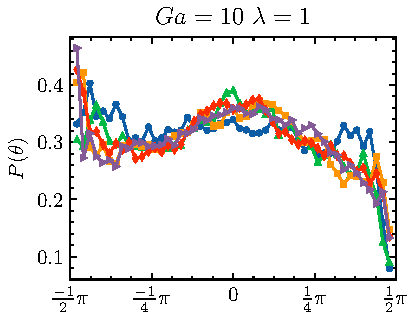
\includegraphics[height=0.3\textwidth]{image/HOMOGENEOUS/fDrop/Pnst_theta_mu_r_1_0_Ga_10.pdf} };
        \node at (0.4\textwidth,0){ 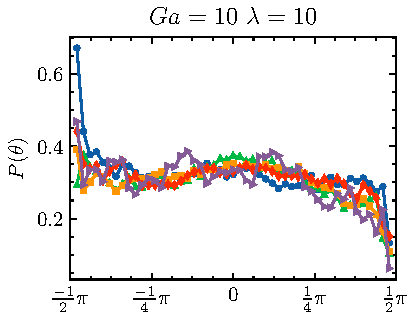
\includegraphics[height=0.3\textwidth]{image/HOMOGENEOUS/fDrop/Pnst_theta_mu_r_0_1_Ga_10.pdf} };
        \node at (0,-0.3\textwidth){ 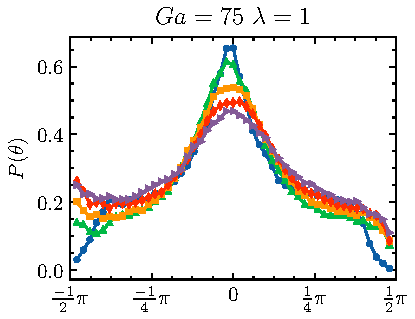
\includegraphics[height=0.3\textwidth]{image/HOMOGENEOUS/fDrop/Pnst_theta_mu_r_1_0_Ga_75.pdf} };
        \node at (0.4\textwidth,-0.3\textwidth){ 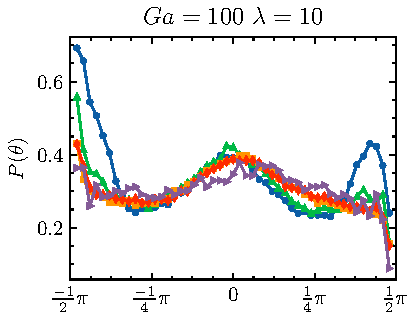
\includegraphics[height=0.3\textwidth]{image/HOMOGENEOUS/fDrop/Pnst_theta_mu_r_0_1_Ga_100.pdf} };
        % \node at (0,-0.6\textwidth){ 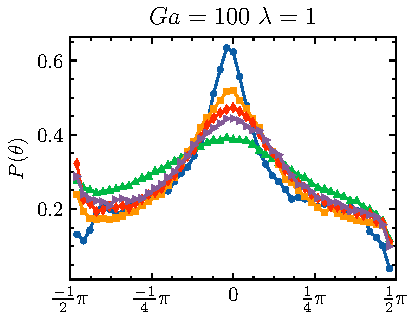
\includegraphics[height=0.3\textwidth]{image/HOMOGENEOUS/fDrop/Pnst_theta_mu_r_1_0_Ga_100.pdf} };
        % \node at (0.4\textwidth,-0.6\textwidth){ 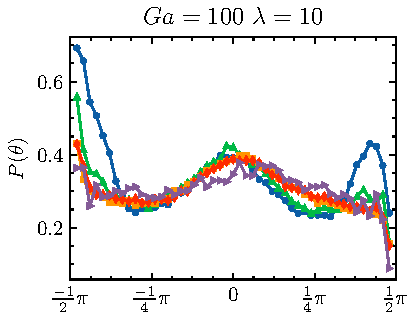
\includegraphics[height=0.3\textwidth]{image/HOMOGENEOUS/fDrop/Pnst_theta_mu_r_0_1_Ga_100.pdf} };
    \end{tikzpicture}
    \caption{Probability density function of the nearest particles : $P_{nst}(\theta)$ for different $Ga$ and $\lambda$. 
    Increasing $Ga$ from top to bottom, (left) $\lambda = 1$ (right) $\lambda = 10$. 
    The symbols correspond to different volume fraction ($\bullet$) $\phi = 1\%$, ($\blacktriangle$) $\phi = 5\%$, ($\blacksquare$) $\phi = 10\%$, ($\blacklozenge$) $\phi = 15\%$ and ($\blacktriangleright$) $\phi = 20\%$.
    (dashed lines) empirical formulas }
    \label{fig:P_nst_theta}
\end{figure}
By using polar coordinate such that $d \textbf{r} = r^2 \sin \phi dr d\phi d\theta$ we can further reduce the PDF to the only consideration of the angular dependency $\theta$ or the distance dependency $r$. 
These reduced p.d.f can be computed as follow, 
\begin{align*}
    P_{nst}(r) 
    &= \int_{-\pi/2}^{\pi/2}\int_{0}^{2\theta} P_{nst}(\textbf{x},\textbf{r},t) \sin \theta  d\phi d\theta\\
    P_{nst}(\theta)
    &= \int_{0}^{\infty}\int_{0}^{2\theta} P_{nst}(\textbf{x},\textbf{r},t) r^2  dr d\phi
\end{align*}
\todo{Check if those formulas are true}
Then $P_{nst}(\theta)$ is the probability that the nearest neighbor of a test particle is inclined at an angle $\theta$ relative to the flow direction. 
We observe that the particles pair becomes oriented with increasing $Ga$ and decreasing volume fraction

On \ref{fig:P_nst_theta} we observe that the particles pair becomes oriented with increasing $Ga$ and decreasing volume fraction.
Indeed, we observe a clear peak of $P_{nst}(\theta)$ at $\theta = \frac{\pi}{2}$. 
It seems that this tendency was also reported for spherical bubble in air-water system \citet{bunner2003effect}. 
Additionally, from \ref{fig:P_nst_theta} we can say that the viscosity ratio $\lambda$ seem to prevent the alignment/clustering of particles denoted by the slightly low peak for $\lambda =10$. 
\todo[inline]{Compart the Orientation with bubbly and solid flows \citet{roghair2011drag}}

\begin{figure}
    \centering
    \begin{tikzpicture}
        \node at (0,0){ 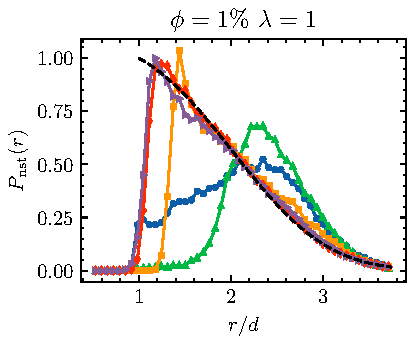
\includegraphics[height=0.3\textwidth]{image/HOMOGENEOUS/fDrop/Pnst_r_mu_r_1_0_PHI_1.pdf} };
        \node at (0.4\textwidth,0){ 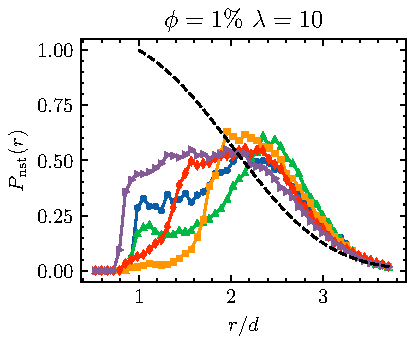
\includegraphics[height=0.3\textwidth]{image/HOMOGENEOUS/fDrop/Pnst_r_mu_r_0_1_PHI_1.pdf} };
        \node at (0,-0.3\textwidth){ 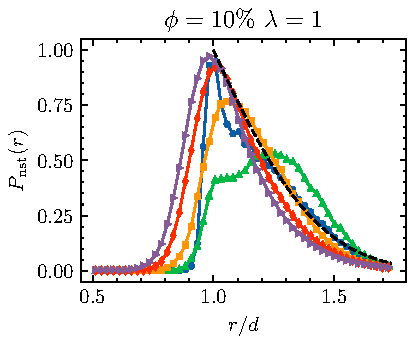
\includegraphics[height=0.3\textwidth]{image/HOMOGENEOUS/fDrop/Pnst_r_mu_r_1_0_PHI_10.pdf} };
        \node at (0.4\textwidth,-0.3\textwidth){ 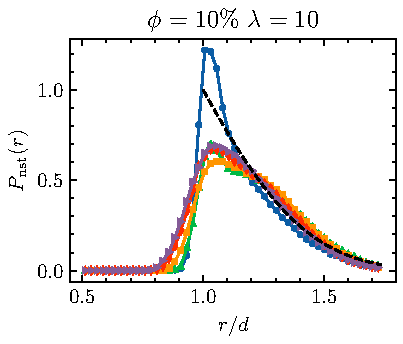
\includegraphics[height=0.3\textwidth]{image/HOMOGENEOUS/fDrop/Pnst_r_mu_r_0_1_PHI_10.pdf} };
        \node at (0,-0.6\textwidth){ 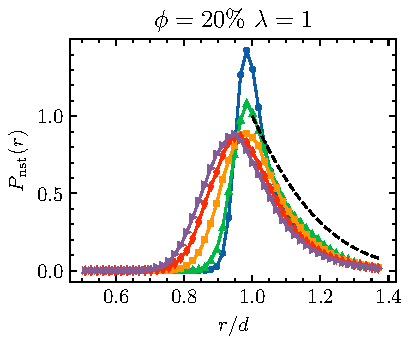
\includegraphics[height=0.3\textwidth]{image/HOMOGENEOUS/fDrop/Pnst_r_mu_r_1_0_PHI_20.pdf} };
        \node at (0.4\textwidth,-0.6\textwidth){ 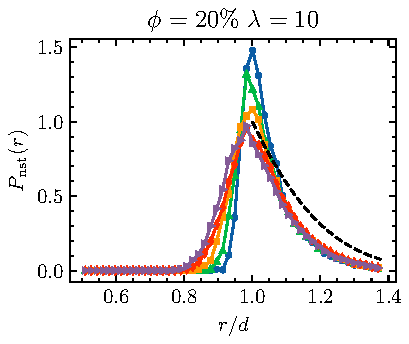
\includegraphics[height=0.3\textwidth]{image/HOMOGENEOUS/fDrop/Pnst_r_mu_r_0_1_PHI_20.pdf} };
    \end{tikzpicture}
    \caption{Radial probability density function : $P_{nst}(r)$ for different $\phi$ and $\lambda$. 
    Increasing $\phi$ from top to bottom, (left) $\lambda = 1$ (right) $\lambda = 10$. 
    The symbols correspond to different Galileo number ($\bullet$) $Ga = 10$, ($\blacktriangle$) $Ga = 25$, ($\blacksquare$) $Ga = 50$, ($\blacklozenge$) $Ga = 75$ and ($\blacktriangleright$) $Ga = 100$.
    (dashed lines) Theoretical formula \ref{eq:P_nst_r}}
    \label{fig:P_nst_r}
\end{figure}
Note that for solid spherical particle in the dilute regime a theoretical formula for $P_{nst}(r)$ can be found assuming completely random distribution and no interactions nor overlap between particles \citep{zhang2021ensemble}, it reads, 
\begin{equation*}
    P_\text{nst}^\text{th}(r) = n_p e^{-4 \pi n_p (r^3 - d^3)/3}.
    \label{eq:P_nst_r}
\end{equation*}
It is evident that all the distribution presented \ref{fig:P_nst_r} have a peak at $r > 1$ where the theoretical formula  predict a peak at $r=1$. 
This is obviously due to the fact that we are in presence of particles interaction which tends to repulse the particles from each others and therefore to shift the distribution to the left. 
What is more interesting is that for $\lambda = 1$ at low volume fraction and high \textit{Galileo} we are able to recover approximately the random particle distribution $P_\text{nst}^\text{th}$ with our numerical results. 
Whereas for $\lambda = 10$ the particle are relatively maintained far from  each other as depicted \ref{fig:P_nst_r}(right). 
We can stipulate that for high viscosity ratio the particles have a tendency to generate more particle fluid mediated interaction as demonstrated by the flow lines \ref{fig:Stream}.


\subsection{Nearest-particle average fluid velocity}
Objectives : 
\begin{itemize}
    \item Problematic "How to analyse the flow around a particle in average"
    \item First : present the averaged the nearest particles' statistics method. And how to compute the nearest averaged velocity fields $\nstavg{\textbf{u}}$.
    \item Present the flowlines and show that for $\phi = 5 \rightarrow 20\%$ we observe that a vertical symmetry arise.
    \item Explain how this field it is related to the velocity fluctuation with \ref{eq:def_uu}
    \item Conclude that these velocity fields represent the PWFs since it represent the mean wakes \citep{du2022analysis}.  
    \item Additionally, some comment can be made regarding the shape of the particle thanks to the contour lines. 
    \item Approach these flow fields by analytical solution of potential flow to obtain an analytical solution for teh reyolds stress. 
\end{itemize}

Presently, we wish to investigate the  averaged flow structure around a fluid particle.
To obtain such a field we make use of the nearest particle statistics recently introduced by \citet{zhang2021stress}. 
We introduce $\nstavg{\textbf{u}}(\textbf{x},\textbf{r})$ as the velocity fields at \textbf{x} knowing there is a particles center of mass located at \textbf{r}.
Additionally, this particle is the nearest particle among all to the point \textbf{x}.  
Formally, this conditional average can be written as, 
\begin{equation}
    \nstavg{\textbf{u}}(\textbf{x},\textbf{r})=\frac{1}{P_{nst}(\textbf{x},\textbf{r})} 
    \int \textbf{u}(\textbf{x},\CC,t) 
    \sum_{\alpha}\delta(\textbf{x}+\textbf{r}-\textbf{x}^\alpha(\CC,t)) h_{\alpha}(\CC,\textbf{x},t) d\mathscr{P} 
    \label{eq:q_nst_avg}
\end{equation}
where $P_{nst}(\textbf{x},\textbf{r})$ is defined as,  
\begin{equation}
    P_{nst}(\textbf{x},\textbf{r})= 
    \int
    \sum_{\alpha}\delta(\textbf{x}+\textbf{r}-\textbf{x}^\alpha(\CC,t)) 
    h_\alpha(\CC,\textbf{x},t) d\mathscr{P}. 
    \label{eq:P_nsti}
\end{equation}
which is the probability of finding a particle center of mass at a distance \textbf{r} from the point \textbf{x} knowing that this particle is the nearest neighbor to the points \textbf{x}. 
The function $h_\alpha$ is defined such that, $h_\alpha = 1/N^p$ if $\alpha$ is the nearest particle to \textbf{x} and $0$ if not, where $N^p$ is the total number of nearest neighbor.
Indeed, the point \textbf{x} at mid-distance from two particles posses two nearest neighbors by definition, thus $N(\textbf{x},\CC,t) = 2$ in this case. 

\todo[inline]{Include the numerical computaiton of $\nstavg{\textbf{u}}$.  }

\ref{fig:Stream} shows the streamline of the field $\nstavg{\textbf{u}}(\textbf{x},\textbf{r})$ for three volume fractions. 
We clearly observe the induced wake of the particles centered at the origin. 

\begin{figure}[h!]
    \centering
    \begin{tikzpicture}
        \node (img) at (0,0)  {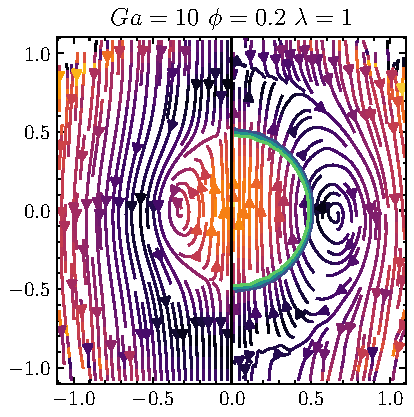
\includegraphics[height=0.3\textwidth]{image/HOMOGENEOUS/Stream/Stream_PHI_20_Ga_10_l_1.pdf}};
        \node (img) at (0.3\textwidth,0)  {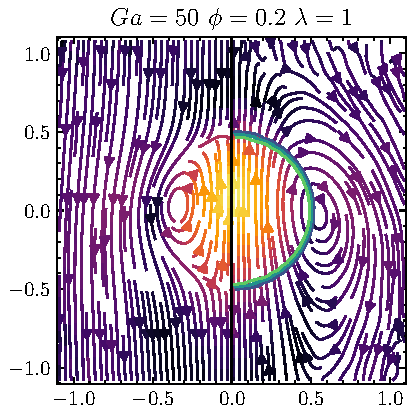
\includegraphics[height=0.3\textwidth]{image/HOMOGENEOUS/Stream/Stream_PHI_20_Ga_50_l_1.pdf}};
        \node (img) at (0.6\textwidth,0)  {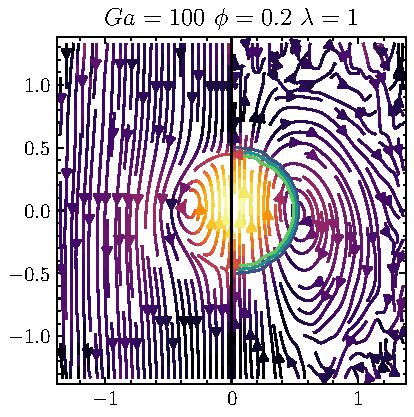
\includegraphics[height=0.3\textwidth]{image/HOMOGENEOUS/Stream/Stream_PHI_20_Ga_100_l_1.pdf}};
        \node (img) at (0,-0.3\textwidth)  {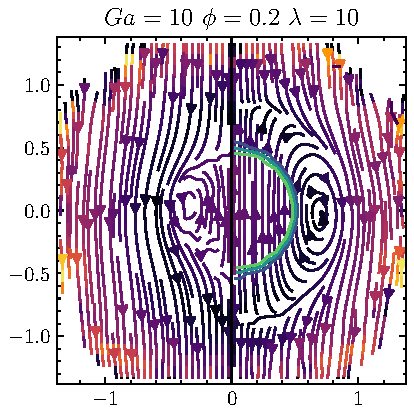
\includegraphics[height=0.3\textwidth]{image/HOMOGENEOUS/Stream/Stream_PHI_20_Ga_10_l_10.pdf}};
        \node (img) at (0.3\textwidth,-0.3\textwidth)  {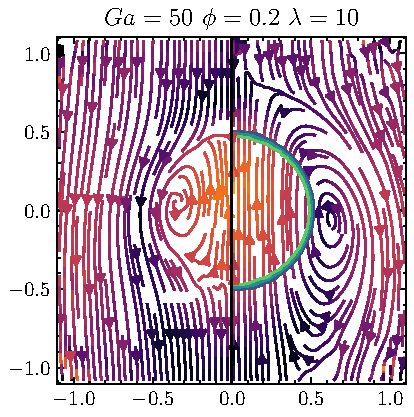
\includegraphics[height=0.3\textwidth]{image/HOMOGENEOUS/Stream/Stream_PHI_20_Ga_50_l_10.pdf}};
        \node (img) at (0.6\textwidth,-0.3\textwidth)  {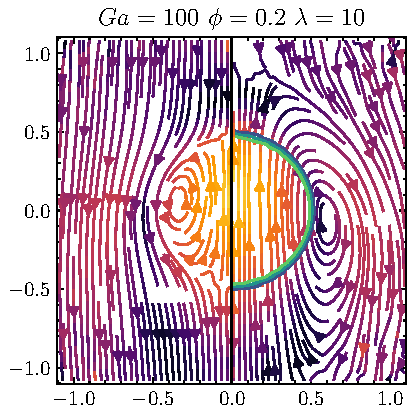
\includegraphics[height=0.3\textwidth]{image/HOMOGENEOUS/Stream/Stream_PHI_20_Ga_100_l_10.pdf}};
        \node (img) at (0,-0.6\textwidth)  {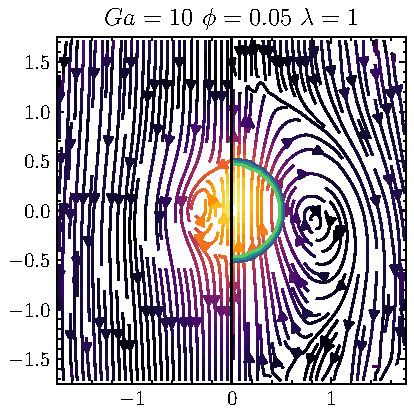
\includegraphics[height=0.3\textwidth]{image/HOMOGENEOUS/Stream/Stream_PHI_5_Ga_10_l_1.pdf}};
        \node (img) at (0.3\textwidth,-0.6\textwidth)  {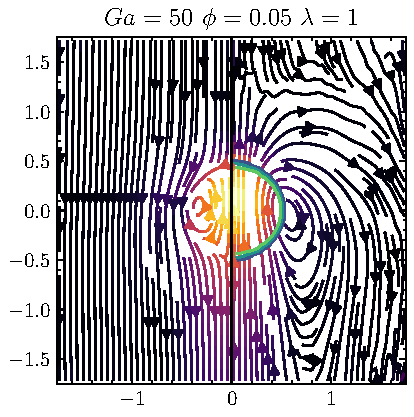
\includegraphics[height=0.3\textwidth]{image/HOMOGENEOUS/Stream/Stream_PHI_5_Ga_50_l_1.pdf}};
        \node (img) at (0.6\textwidth,-0.6\textwidth)  {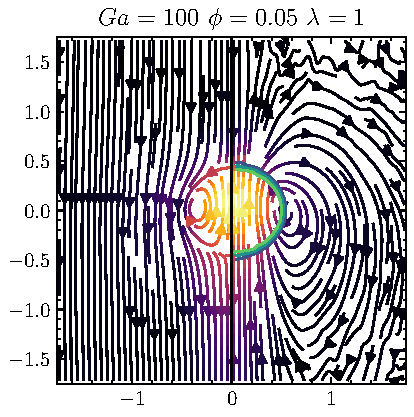
\includegraphics[height=0.3\textwidth]{image/HOMOGENEOUS/Stream/Stream_PHI_5_Ga_100_l_1.pdf}};
        \node (img) at (0,-0.9\textwidth)  {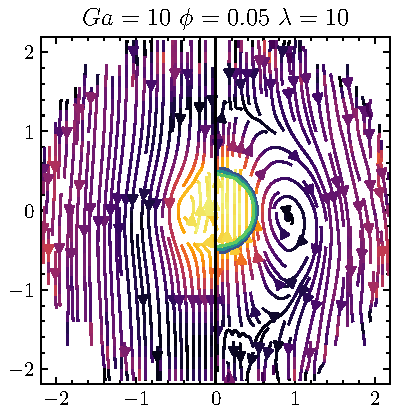
\includegraphics[height=0.3\textwidth]{image/HOMOGENEOUS/Stream/Stream_PHI_5_Ga_10_l_10.pdf}};
        \node (img) at (0.3\textwidth,-0.9\textwidth)  {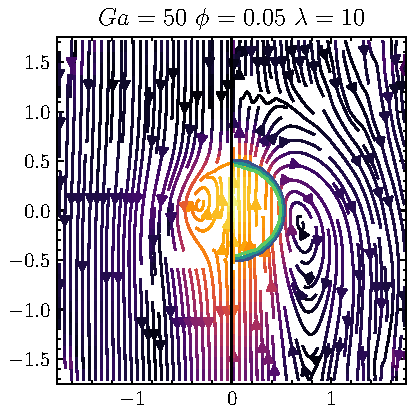
\includegraphics[height=0.3\textwidth]{image/HOMOGENEOUS/Stream/Stream_PHI_5_Ga_50_l_10.pdf}};
        \node (img) at (0.6\textwidth,-0.9\textwidth)  {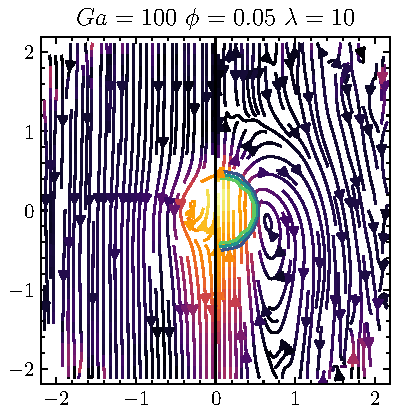
\includegraphics[height=0.3\textwidth]{image/HOMOGENEOUS/Stream/Stream_PHI_5_Ga_100_l_10.pdf}};
    \end{tikzpicture}
    \caption{Nearest particle averaged velocity $\nstavg{\textbf{u}}(\textbf{r})$ for  $\phi = 5\%$ and $20\%$.
    Green lines : contour plots of the nearest averaged indicator function $\nstavg{\chi_d}(\textbf{r})$ (it represent the mean shape of the particles)}
    \label{fig:Stream}
\end{figure}
% \begin{figure}[h!]
%     \centering
%     \begin{tikzpicture}
%         \node (img) at (0,0)  {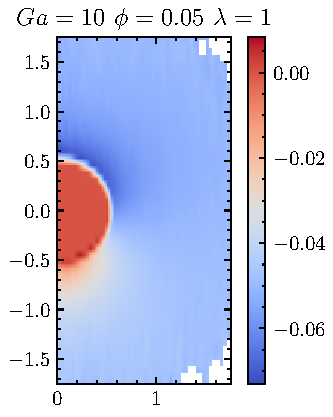
\includegraphics[height=0.4\textwidth]{image/HOMOGENEOUS/Stream/P_PHI_5_Ga_10_l_1.pdf}};
%         \node (img) at (0.3\textwidth,0)  {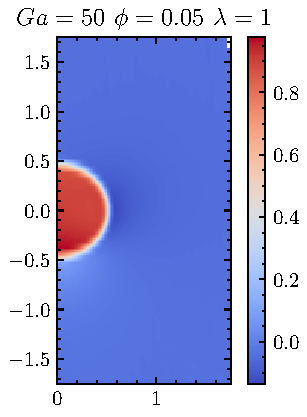
\includegraphics[height=0.4\textwidth]{image/HOMOGENEOUS/Stream/P_PHI_5_Ga_50_l_1.pdf}};
%         \node (img) at (0.6\textwidth,0)  {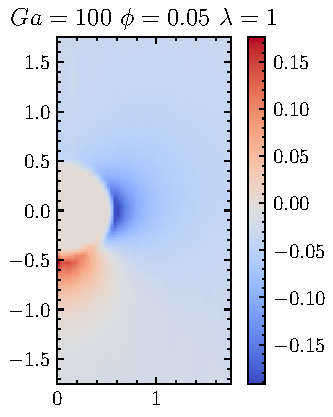
\includegraphics[height=0.4\textwidth]{image/HOMOGENEOUS/Stream/P_PHI_5_Ga_100_l_1.pdf}};
%         \node (img) at (0,0.4\textwidth)  {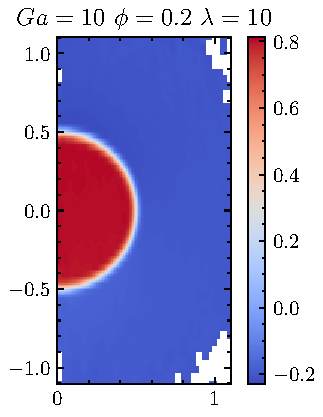
\includegraphics[height=0.4\textwidth]{image/HOMOGENEOUS/Stream/P_PHI_20_Ga_10_l_10.pdf}};
%         \node (img) at (0.3\textwidth,0.4\textwidth)  {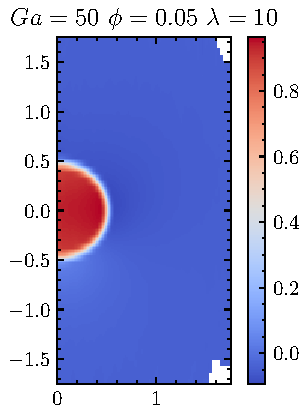
\includegraphics[height=0.4\textwidth]{image/HOMOGENEOUS/Stream/P_PHI_5_Ga_50_l_10.pdf}};
%         \node (img) at (0.6\textwidth,0.4\textwidth)  {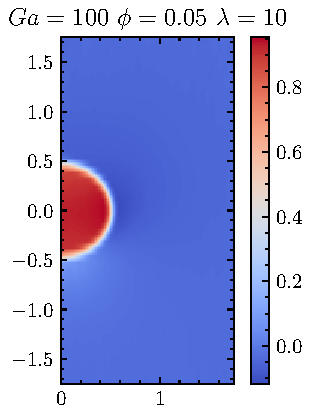
\includegraphics[height=0.4\textwidth]{image/HOMOGENEOUS/Stream/P_PHI_5_Ga_100_l_10.pdf}};
%     \end{tikzpicture}
%     \caption{Nearest particle averaged pressure $\nstavg{p}(\textbf{r})$ normalized by the Laplace pressure $4 \gamma /d$ for  $\phi = 5\%$ and $20\%$}
%     \label{fig:Stream}
% \end{figure}
\begin{figure}[h!]
    \centering
    \begin{tikzpicture}
        \node (img) at (0,0)  {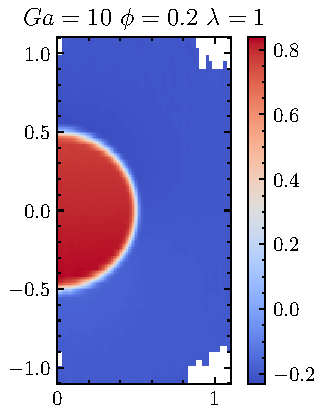
\includegraphics[height=0.3\textwidth]{image/HOMOGENEOUS/Stream/P_PHI_20_Ga_10_l_1.pdf}};
        \node (img) at (0.3\textwidth,0)  {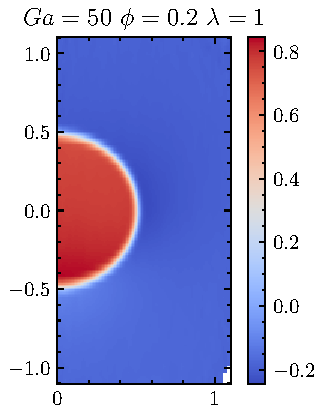
\includegraphics[height=0.3\textwidth]{image/HOMOGENEOUS/Stream/P_PHI_20_Ga_50_l_1.pdf}};
        \node (img) at (0.6\textwidth,0)  {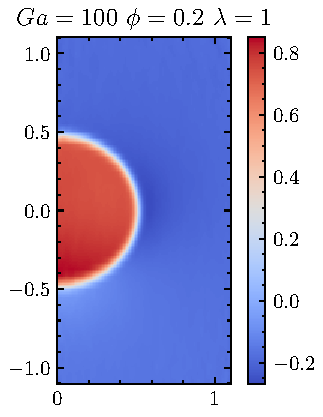
\includegraphics[height=0.3\textwidth]{image/HOMOGENEOUS/Stream/P_PHI_20_Ga_100_l_1.pdf}};
        \node (img) at (0,-0.3\textwidth)  {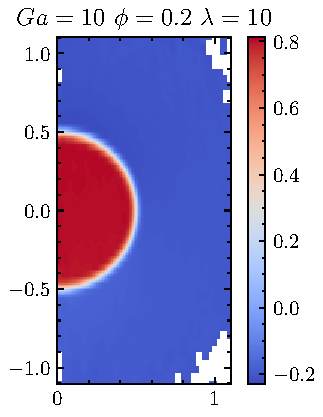
\includegraphics[height=0.3\textwidth]{image/HOMOGENEOUS/Stream/P_PHI_20_Ga_10_l_10.pdf}};
        \node (img) at (0.3\textwidth,-0.3\textwidth)  {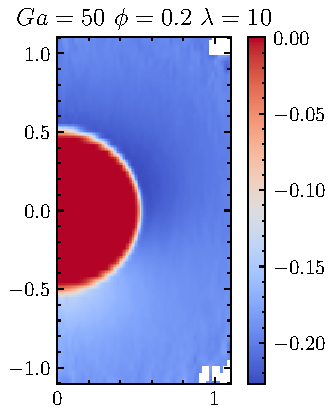
\includegraphics[height=0.3\textwidth]{image/HOMOGENEOUS/Stream/P_PHI_20_Ga_50_l_10.pdf}};
        \node (img) at (0.6\textwidth,-0.3\textwidth)  {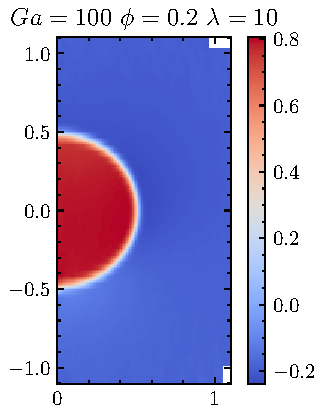
\includegraphics[height=0.3\textwidth]{image/HOMOGENEOUS/Stream/P_PHI_20_Ga_100_l_10.pdf}};
        \node (img) at (0,-0.6\textwidth)  {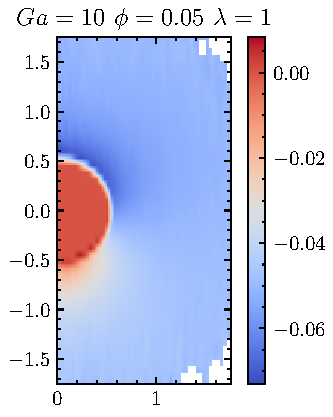
\includegraphics[height=0.3\textwidth]{image/HOMOGENEOUS/Stream/P_PHI_5_Ga_10_l_1.pdf}};
        \node (img) at (0.3\textwidth,-0.6\textwidth)  {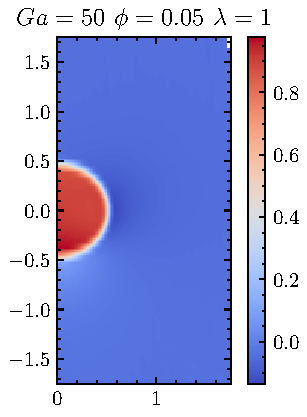
\includegraphics[height=0.3\textwidth]{image/HOMOGENEOUS/Stream/P_PHI_5_Ga_50_l_1.pdf}};
        \node (img) at (0.6\textwidth,-0.6\textwidth)  {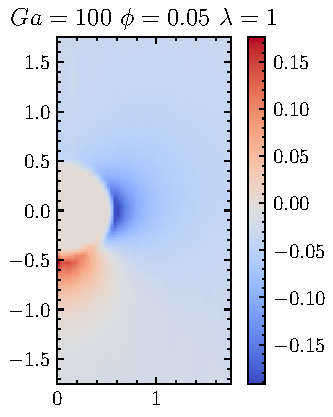
\includegraphics[height=0.3\textwidth]{image/HOMOGENEOUS/Stream/P_PHI_5_Ga_100_l_1.pdf}};
        % \node (img) at (0,-0.9\textwidth)  {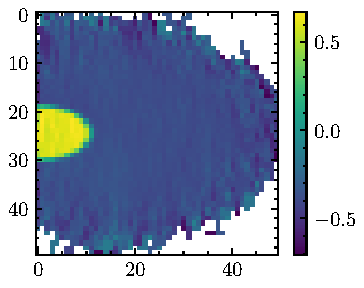
\includegraphics[height=0.3\textwidth]{image/HOMOGENEOUS/Stream/P_PHI_5_Ga_10_l_10.pdf}};
        \node (img) at (0.3\textwidth,-0.9\textwidth)  {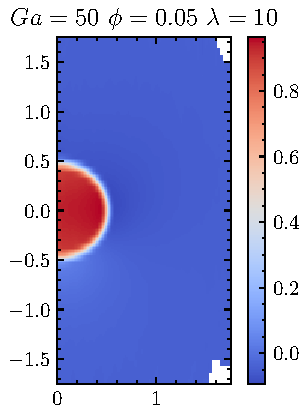
\includegraphics[height=0.3\textwidth]{image/HOMOGENEOUS/Stream/P_PHI_5_Ga_50_l_10.pdf}};
        \node (img) at (0.6\textwidth,-0.9\textwidth)  {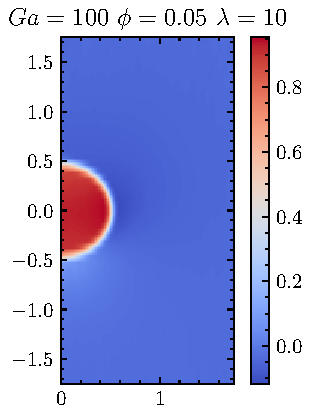
\includegraphics[height=0.3\textwidth]{image/HOMOGENEOUS/Stream/P_PHI_5_Ga_100_l_10.pdf}};
    \end{tikzpicture}
    \caption{Nearest particle averaged pressure $\nstavg{p}(\textbf{r})$ normalized by the Laplace pressure $4 \gamma /d$ for  $\phi = 5\%$ and $20\%$}  
    \label{fig:Stream}
\end{figure}
It is evident from these plots that the induced wake is the averaged wake resulting from the averaged translation of the particles. 
And this averaged wake has a tendency to be asymmetrical for low volume fraction and symmetrical for higher ones. 
Additionally, form basic mathematical consideration on the average operators we can demonstrate that :
\begin{multline*}
    \avg{\chi_k \textbf{u}'_k\textbf{u}'_k}(\textbf{x},t)
    + \phi_k \textbf{u}_k\textbf{u}_k
    = \\
    \underbrace{\int (\nstavg{\chi_k \textbf{u}^0_k}  \nstavg{\chi_k \textbf{u}^0_k} / (\nstavg{\chi_k})  P_{nst}(\textbf{x},t,\textbf{r}) d\textbf{r} }_\text{PWFs}
    +\underbrace{\int \nstavg{\chi_k \textbf{v}_k^0\textbf{v}_k^0}  P_{nst}(\textbf{x},t,\textbf{r}) d\textbf{r}}_\text{WIA}
    \label{eq:def_uu}
\end{multline*}
where, $\textbf{v}_k^0  = \textbf{u}_k^0 - \nstavg{\chi_k \textbf{u}^0_k} / \nstavg{\chi_k}$ is the fluctuation of the local velocity relative to the nearest averaged value. 
Consequently, we can decompose the ensemble averaged fluid velocity fluctuations with a first term representing the variance of $\nstavg{\textbf{u}}$ around the mean $\textbf{u}_k$, and a second term representing the variance of $\textbf{u}^0_k$ around the mean  $\nstavg{\textbf{u}}$. 

There are two phenomena causing velocity fluctuations in the liquid:
the agitation resulting from wakes and their collective interactions [wake-induced agitation (WIA)], and the non-turbulent fluctuations resulting from averaged wakes and potential flows around bubbles [potential flow and averaged wake fluctuations (PWFs)].
As a matter of fact in the phase space of $\nstavg{\textbf{u}}(\textbf{r})$ the bubble is fixed at the origin thus we recover the velocity fields representing what is called the PWFs. 
In their study \citet{du2022analysis} carry out transient simulation with fixed particles to recover the PWFs components here we show that a single simulation permit us to recover WIA and PWFs by the mean of the nearest particles' statistics. 

\todo[inline]{make the link with drag force/drag coef  \citet{dandy1989buoyancy}}
\todo[inline]{make the link with velocity fluctuation \citet{almeras2021statistics}}





\subsection{Nearest averaged particle center of mass velocity}
\subsubsection{Nearest averaged particle center of mass velocity in the dispersed phase reference frame}
\begin{equation}
    \nstavg{\textbf{u}^i}=\frac{1}{P_{nst}(\textbf{x},\textbf{r},t)} 
    \int \sum_{i}\delta(\textbf{x}-\textbf{x}^i(\CC,t))
    \sum_{j\neq i}\delta(\textbf{x}+\textbf{r}-\textbf{x}^j(\CC,t)) 
    % \delta(t+a-t_c^{ij}(\CC,t)) 
    h_{ij}(\CC,t) 
    \textbf{u}^i(\CC,t)
    d\mathscr{P} 
    - \textbf{u}_p
\end{equation}
\subsubsection{Nearest averaged particle center of mass relative velocity}
\begin{equation}
    \nstavg{\textbf{w}}=\frac{1}{P_{nst}(\textbf{x},\textbf{r},t)} 
    \int \sum_{i}\delta(\textbf{x}-\textbf{x}^i(\CC,t))
    \sum_{j\neq i}\delta(\textbf{x}+\textbf{r}-\textbf{x}^j(\CC,t)) 
    % \delta(t+a-t_c^{ij}(\CC,t)) 
    h_{ij}(\CC,t) 
    (\textbf{u}^i(\CC,t) - \textbf{u}^j(\CC,t))
    d\mathscr{P} 
\end{equation}


\begin{figure}[h!]
    \centering
    \begin{tikzpicture}
        \node (img) at (0,0)  {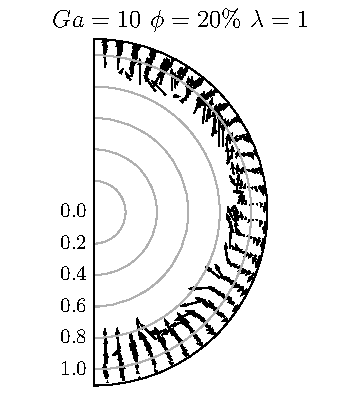
\includegraphics[height=0.3\textwidth]{image/HOMOGENEOUS/fDrop/U_l_1_Ga_10_PHI_20.pdf}};
        \node (img) at (0.3\textwidth,0)  {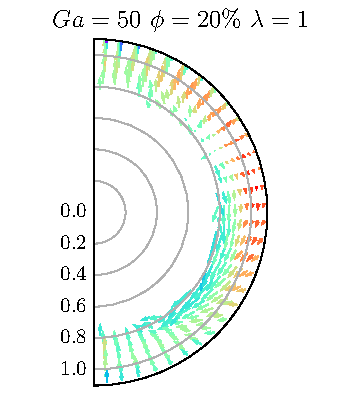
\includegraphics[height=0.3\textwidth]{image/HOMOGENEOUS/fDrop/U_l_1_Ga_50_PHI_20.pdf}};
        \node (img) at (0.6\textwidth,0)  {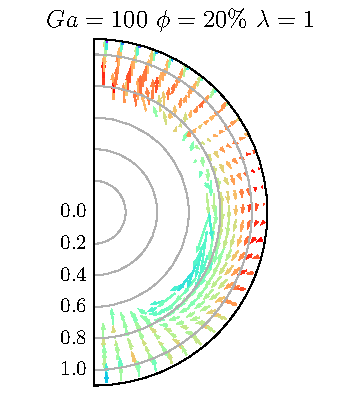
\includegraphics[height=0.3\textwidth]{image/HOMOGENEOUS/fDrop/U_l_1_Ga_100_PHI_20.pdf}};
        \node (img) at (0,-0.3\textwidth)  {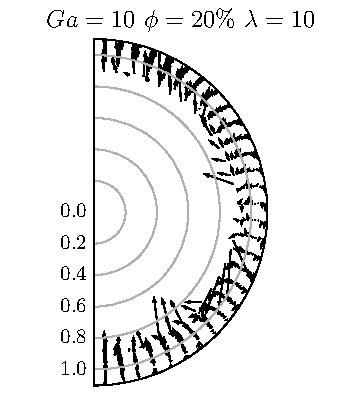
\includegraphics[height=0.3\textwidth]{image/HOMOGENEOUS/fDrop/U_l_10_Ga_10_PHI_20.pdf}};
        \node (img) at (0.3\textwidth,-0.3\textwidth)  {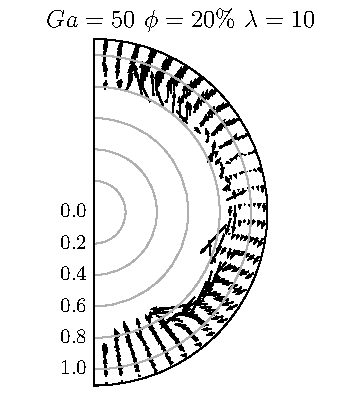
\includegraphics[height=0.3\textwidth]{image/HOMOGENEOUS/fDrop/U_l_10_Ga_50_PHI_20.pdf}};
        \node (img) at (0.6\textwidth,-0.3\textwidth)  {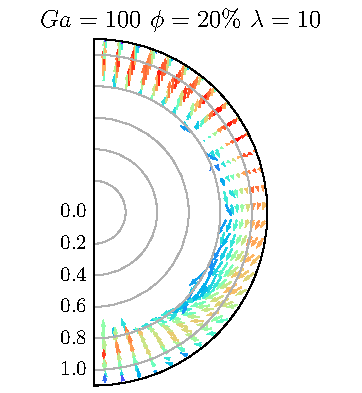
\includegraphics[height=0.3\textwidth]{image/HOMOGENEOUS/fDrop/U_l_10_Ga_100_PHI_20.pdf}};
        \node (img) at (0,-0.6\textwidth)  {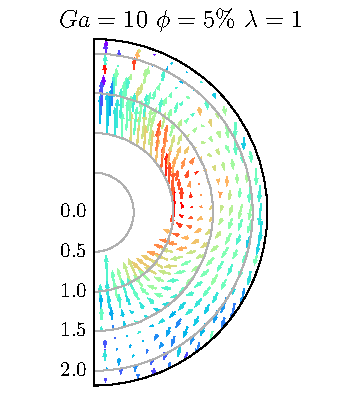
\includegraphics[height=0.3\textwidth]{image/HOMOGENEOUS/fDrop/U_l_1_Ga_10_PHI_5.pdf}};
        \node (img) at (0.3\textwidth,-0.6\textwidth)  {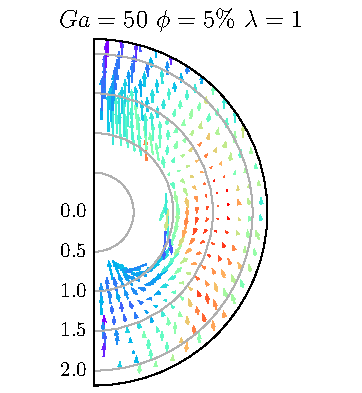
\includegraphics[height=0.3\textwidth]{image/HOMOGENEOUS/fDrop/U_l_1_Ga_50_PHI_5.pdf}};
        \node (img) at (0.6\textwidth,-0.6\textwidth)  {\includegraphics[height=0.3\textwidth]{image/HOMOGENEOUS/fDrop/U_l_1_Ga_75_PHI_5.pdf}};
        \node (img) at (0,-0.9\textwidth)  {\includegraphics[height=0.3\textwidth]{image/HOMOGENEOUS/fDrop/U_l_10_Ga_10_PHI_5.pdf}};
        \node (img) at (0.3\textwidth,-0.9\textwidth)  {\includegraphics[height=0.3\textwidth]{image/HOMOGENEOUS/fDrop/U_l_10_Ga_50_PHI_5.pdf}};
        \node (img) at (0.6\textwidth,-0.9\textwidth)  {\includegraphics[height=0.3\textwidth]{image/HOMOGENEOUS/fDrop/U_l_10_Ga_75_PHI_5.pdf}};
    \end{tikzpicture}
    \caption{Nearest particle averaged pressure velocity $\nstavg{\textbf{u}^i}(\textbf{r}) - \textbf{u}_p$ }  
    \ref{fig:u_nst}
\end{figure}
\begin{figure}[h!]
    \centering
    \begin{tikzpicture}
        \node (img) at (0,0)  {\includegraphics[height=0.3\textwidth]{image/HOMOGENEOUS/fDrop/U_rel_l_1_Ga_10_PHI_20.pdf}};
        \node (img) at (0.3\textwidth,0)  {\includegraphics[height=0.3\textwidth]{image/HOMOGENEOUS/fDrop/U_rel_l_1_Ga_50_PHI_20.pdf}};
        \node (img) at (0.6\textwidth,0)  {\includegraphics[height=0.3\textwidth]{image/HOMOGENEOUS/fDrop/U_rel_l_1_Ga_100_PHI_20.pdf}};
        \node (img) at (0,-0.3\textwidth)  {\includegraphics[height=0.3\textwidth]{image/HOMOGENEOUS/fDrop/U_rel_l_10_Ga_10_PHI_20.pdf}};
        \node (img) at (0.3\textwidth,-0.3\textwidth)  {\includegraphics[height=0.3\textwidth]{image/HOMOGENEOUS/fDrop/U_rel_l_10_Ga_50_PHI_20.pdf}};
        \node (img) at (0.6\textwidth,-0.3\textwidth)  {\includegraphics[height=0.3\textwidth]{image/HOMOGENEOUS/fDrop/U_rel_l_10_Ga_100_PHI_20.pdf}};
        \node (img) at (0,-0.6\textwidth)  {\includegraphics[height=0.3\textwidth]{image/HOMOGENEOUS/fDrop/U_rel_l_1_Ga_10_PHI_5.pdf}};
        \node (img) at (0.3\textwidth,-0.6\textwidth)  {\includegraphics[height=0.3\textwidth]{image/HOMOGENEOUS/fDrop/U_rel_l_1_Ga_50_PHI_5.pdf}};
        \node (img) at (0.6\textwidth,-0.6\textwidth)  {\includegraphics[height=0.3\textwidth]{image/HOMOGENEOUS/fDrop/U_rel_l_1_Ga_75_PHI_5.pdf}};
        \node (img) at (0,-0.9\textwidth)  {\includegraphics[height=0.3\textwidth]{image/HOMOGENEOUS/fDrop/U_rel_l_10_Ga_10_PHI_5.pdf}};
        \node (img) at (0.3\textwidth,-0.9\textwidth)  {\includegraphics[height=0.3\textwidth]{image/HOMOGENEOUS/fDrop/U_rel_l_10_Ga_50_PHI_5.pdf}};
        \node (img) at (0.6\textwidth,-0.9\textwidth)  {\includegraphics[height=0.3\textwidth]{image/HOMOGENEOUS/fDrop/U_rel_l_10_Ga_75_PHI_5.pdf}};
    \end{tikzpicture}
    \caption{Nearest particle averaged pressure velocity $\nstavg{\textbf{w}}(\textbf{r})$ }  
    \ref{fig:w_nst}
\end{figure}